% IN THIS SECTION SHOW SOME OF OUR TRANSLATED CODE... AND WALK THROUGH IT THE SAME WAY YOU DID WITH THE CONCEPT IN RESOLVE. BUT BEFORE YOU DO THAT, SHOW THE PICTURE (The one thats already here showing high level relationships and update it!).
\section{Implementation}\label{sec:impl}
Development of our C translation tool can be logically partitioned into three distinct phases: 
\begin{enumerate}
\item Arriving at a translation model (or, strategy) for an accurate C representation of RESOLVE.
\item Implementing suitable mechanisms for carrying out the C code generation process.
\item Creation of a memory manager capable of safely allocating and freeing dynamic memory required by the generated code.
\end{enumerate}
We conclude this section with a demonstration of each of these phases working in tandem on the LED component discussed in Section \ref{sec:specifiying}. 

\subsection{C Translation Model}
One of the primary challenges in translating from RESOLVE to C is finding a suitable C analog for each RESOLVE module and the constructs allowable in each. Indeed, since we are dealing with an environment where functional correctness is a primary concern, it is important that the code generated by our tool represents as closely as possible the original RESOLVE source. In an effort to make such considerations, at the highest level, the C code we generate makes special considerations for concepts, facilities, and realizations. This scheme is depicted in Figure \ref{fig:relationship} and briefly summarized throughout Sections \ref{sec:conceptoverview} - \ref{sec:facilitiesrealizations}.

\begin{figure}
\begin{center}
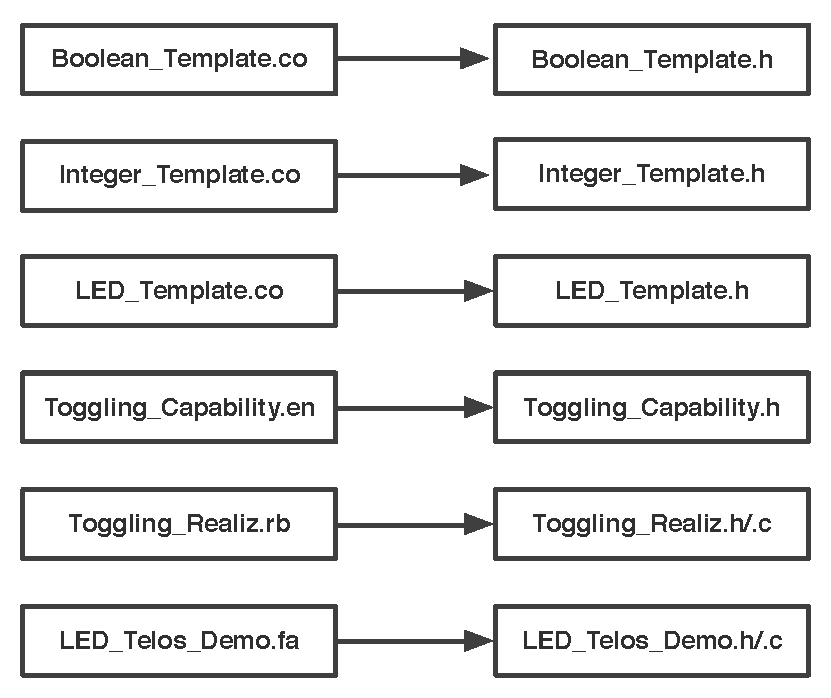
\includegraphics[scale=.55]{figs/relationship.pdf}
\end{center}
\caption{Relationship between RESOLVE module types and the C code generated from each.}
\label{fig:relationship}
\end{figure}

\begin{figure*}[!htb]
\begin{center}
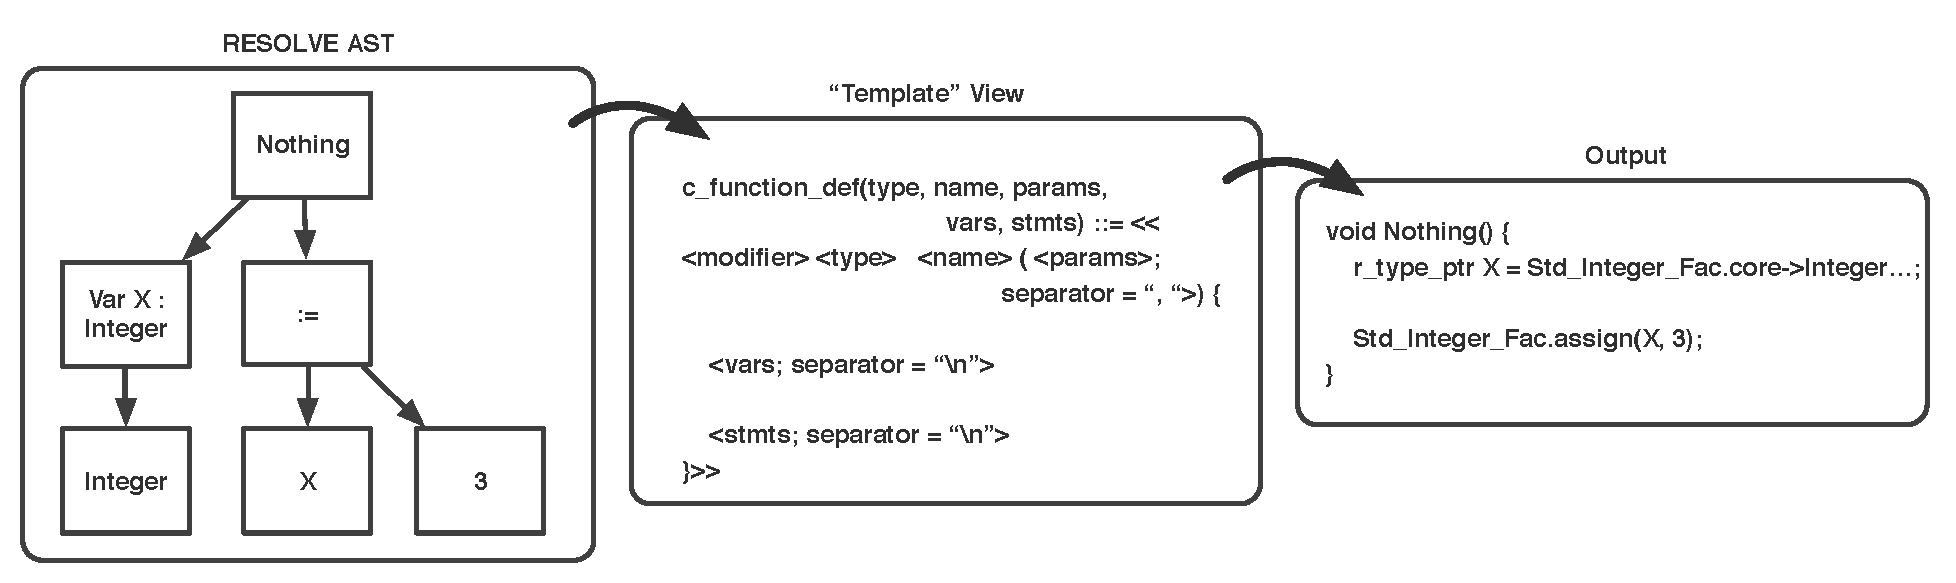
\includegraphics[scale=.54]{figs/ast_traversal2.pdf}
\end{center}
\caption{The general flow of information from the AST (first), to user defined templates (middle), ending with formed output (last).}
\label{fig:ast}
\end{figure*}

\subsubsection{Concepts}
\label{sec:conceptoverview}
Concept modules produce a single .h file, which provide function pointers for the operations specified in the original concept, as well as structs representing each user defined type. 

\subsubsection{Facilities}
\label{sec:facilitiesoverview}
Facilities produce an .h/.c pair: The header .h declares both a ``create" and ``destroy" method which, taken together, encapsulates the creation and destruction of all global variables used within the facility. The .c provides an implementation of these methods.  Note that these create and destroy methods are only responsible for freeing \textit{global} variables -- meaning all other translated functions are responsible for deallocating their own local variables. 

\subsubsection{Realizations}
\label{sec:facilitiesrealizations}
We treat realizations of concepts and enhancements slightly different than facility modules. While a .h/.c pair is still produced, the create method designated in the header for realizations is designed to create instances of all types specified by the concept, while the destroy method deallocates these types -- as opposed to simply destroying user created globals.

\subsection{Translator Implementation}

Translation itself occurs over the course of a traversal of RESOLVE's abstract syntax tree (AST) -- an intermediate representation of RESOLVE code. The traversal mechanism utilized is a derivative of the visitor pattern that provides a pre post traversal over all nodes in the tree. 

%\subsubsection{AST Traversal}
%Translation is performed over the course of a traversal of RESOLVE's abstract syntax tree (AST). The traversal mechanism used is a dervivative of the visitor pattern that provides a SAX-dom style pre-post traversal over all nodes in the tree. Thus, for any given node present, a total of two visits occur: One corresponding to the node being `hit' during the pre traversal stage, and one for the post. 

To illustrate the general process of producing runnable C from RESOLVE code, consider the following dummy operation:

\begin{verbatim}
Operation Nothing(); Procedure
        Var X : Integer;
        X := 3;
end Nothing;
\end{verbatim}

Shown in Figure \ref{fig:ast} is a high level depiction of steps taken in translating this operation to C. The first box depicts the AST of \texttt{Nothing}, where nodes are represented as boxes labeled by the constructs they contain. Throughout the walk of this tree, useful information such as the operation's name, ``Nothing", are extracted from nodes, and added as parameters to user defined templates\footnote{A template can simply be thought of as a ``document with holes" which the user choses when and how to fill.}, in this case: \texttt{c\_function\_def}.

In the context of RESOLVE to C translation, these templates, when filled during the aforementioned pre-post visitor traversal of RESOLVE's AST, help simplify the task of producing complicated, arbitrarily nested blocks of structured C output by keeping translation logic strictly within the C translator, and output logic strictly within the templates.

That is, the only actual work being performed within the C translator is forwarding information gathered from individual treenodes, to a series of externally defined templates. This allows us to exploit (in design pattern parlance \cite{krasner:1988}) a strict model view controller (MVC) separation in the translator's codebase between the mechanism that does the AST visiting (controller), the tree nodes from which we're adding information to templates (model), and the external file containing all available C language templates which shape our output (view).

We feel this approach lends itself well to the challenge discussed in this paper, as this separation allows us to easily iterate changes to our generated C code without needing to concern ourselves with the Java written inside the compiler itself.

%%%%%%%%%%%%%%%%%%%%%%%
%           Memory Allocation Section              %
%%%%%%%%%%%%%%%%%%%%%%%
\subsection{Strategy for Dynamic Memory Allocation}\label{sec:mem}

Any model seeking to convert RESOLVE to a lower level representation such as C demands a strategy for handling memory utilized by the generated code. While dynamic allocation is typically the norm, it is not however the first choice for embedded applications. With the Telosb mote constrained to 10kB of RAM, developers targeting embedded platforms tend to favor static memory allocation over dynamic, due the memory efficiency it affords. 

%Many programs however benefit greatly from dynamic memory allocation not only in terms of clarity and straightforwardness, but in our case: Accurately modeling exactly what the code being executed is doing. 
%NesC, for example, while giving the illusion of dynamic allocation, behind the scenes actually performs static allocation 

In spite of this, our reasoning for choosing to pursue dynamic allocation over static, rests in the language itself. Being a language that relies heavily on the notion of formally specified, verifiable objects (components), everything in RESOLVE from the `primitive' types such as booleans and integers, to the more complicated ones such as Stacks and Queues, are modeled, specified, and implemented in the same way: Using the standard component machinery showcased in Section \ref{sec:specifiying}. 

As such, even the simplest RESOLVE programs still rely heavily on the notion of objects coming and going. Thus, from a verification perspective, creating a tool that allows our translated code to create and destroy such objects in a manner consistent with the language is an extremely important aspect towards maintaining the ``correct-by-construction" property of our automatically generated C code.

The previous iteration of this tool \cite{regula:2010} achieves static allocation by effectively introducing a second pass to the compiler dedicated to replacing all formal parameters with their corresponding facility-instantiated literal values. This additional, hidden step to compilation is less than ideal in the context of a verifying compiler designed from the ground up to be a single pass system. We feel the work we present here avoids these wrinkles with a dynamic approach.

\subsubsection{Allocation using ``salloc''}

The dynamic allocatior we create for our generated code is \texttt{salloc()}: A first fit memory allocator. Rather than conventional, heap-based allocators, \texttt{salloc()} uses stack memory for allocation. This approach requires that a single fixed block of memory is chosen at compilation. In addition, \texttt{salloc()}, requires a section of meta-data, denoted as a \texttt{block}, for each record in memory. A \texttt{block} holds referential information about neighboring blocks, the size of the record the block maintains, and if the block is free or is in use. Figure~\ref{fig:stack} is an example of the stack after several calls to \texttt{salloc()}.

\begin{figure}[!htb]
%\centering
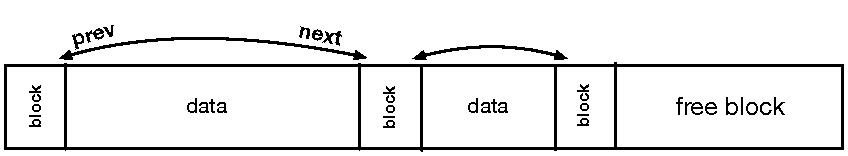
\includegraphics[scale=.55]{figs/stack.pdf}
\caption{Memory allocated with salloc() allocates a block in front of data allocated. Blocks point to their immediate neighbors and hold their size and usage.}

\label{fig:stack}
\end{figure}

\subsubsection{Deallocation using \texttt{sfree}}

A memory allocator must provide a mechanism to release, or free a section of memory in order to indicate that it is not being used and that it may be reallocated. Our \texttt{sfree()} function, which provides this functionality, is illustrated in Figure~\ref{fig:free} -- depicting memory before and after a call to \texttt{sfree()}. 

\begin{figure}[!htb]
%\centering
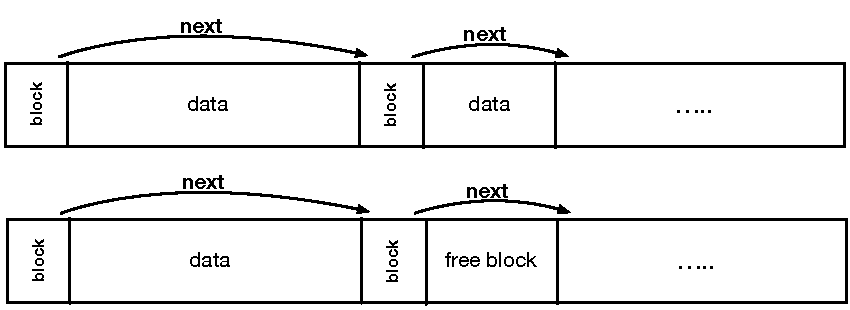
\includegraphics[scale=.55]{figs/sfree.pdf}
\caption{An illustration of sfree.}
\label{fig:free}
\end{figure}

\subsubsection{Optimizing Memory Usage}

A common problem that can occur in memory allocation is fragmentation. During execution, a program can allocate and deallocate memory an arbitrary number of times. Figure~\ref{fig:fragmentation} depicts some of the problems that might arise from this such as a decreased success rate for allocation and increased overall memory usage. The problem is especially magnified on embedded systems, due to their limited memory capacity. We employ two simple optimizations to help reduce this.

\begin{itemize}
\item \textbf{Block splitting:} As shown in Figure~\ref{fig:split}, unused blocks can be repartitioned to the size of memory needed by \texttt{salloc()}.
\item \textbf{Block fusing:}
This technique is applied during deallocation. When memory is deallocated by \texttt{sfree()}, neighboring free blocks containing unused memory are coalesced into a single large block, as shown in Figure~\ref{fig:fuse}.
\end{itemize} 

%The first is block splitting, as shown in Figure~\ref{fig:split}, occurs during allocation. It allows blocks of greater size to be partitioned into the size requested by the allocator. 

%Fusing blocks is another technique used when \texttt{sfree()} is called. When memory is deallocated, neighboring free blocks are coalesced to form a single large block, as shown in Figure~\ref{fig:fuse}. 

\begin{figure}[!htb]
\centering
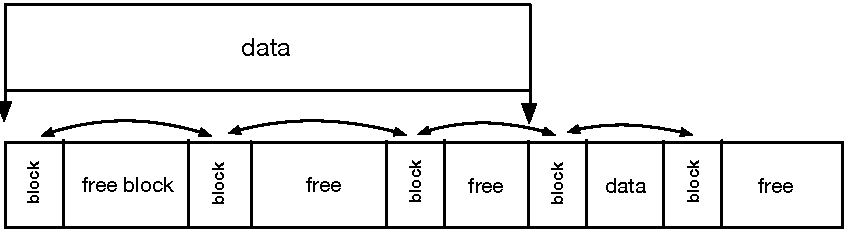
\includegraphics[scale=.55]{figs/fragmentation.pdf}
\caption{Performing naive allocation and deallocations restricts allocatable blocks to those that match the size requested.}
\label{fig:fragmentation}
\end{figure}

\begin{figure}[!htb]
\centering
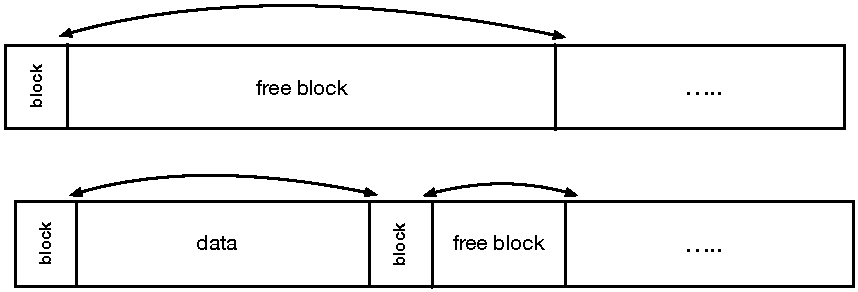
\includegraphics[scale=.55]{figs/split.pdf}
\caption{Splitting creates a block that is the size that the allocator requested, and a new free block with the remainder of memory.}
\label{fig:split}
\end{figure}


\begin{figure}[!htb]
\centering
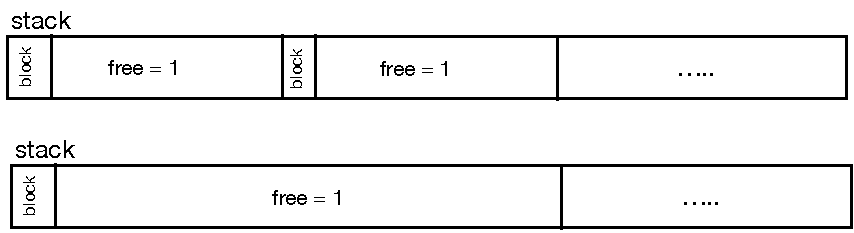
\includegraphics[scale=.55]{figs/fuse.pdf}
\caption{Block fusing. This creates single larger block, decreasing the number of smaller blocks unable to split.}
\label{fig:fuse}
\end{figure}

%
%
